\documentclass[a4paper,10pt]{scrartcl}
\usepackage[utf8]{inputenc}
\usepackage[hyphens]{url}
\usepackage{hyperref}
\usepackage[ngerman]{babel}
\usepackage[T1]{fontenc}
\usepackage{graphicx}
\usepackage[utf8]{inputenc}
\usepackage{lmodern}
\usepackage{geometry}
\usepackage{pgfplots} 
\usepackage{mathrsfs}
\usepackage{mathtools}
\usepackage{listings}
\usepackage{wrapfig}
\usepackage{float}
\usepackage{amsmath}
\usepackage{stmaryrd}
\usepackage{paralist}
\usepackage{color}
\lstset{basicstyle=\normalfont\ttfamily,breaklines=true}


\geometry{paper=a4paper, left=25mm, right=25mm, top=35mm, bottom=35mm}
\hypersetup{
    unicode=false,
    pdftoolbar=true,
    pdfmenubar=true,
    pdffitwindow=false,
    pdfstartview={FitH},
    pdftitle={DataScienceReport},
    pdfauthor={PaSeDa},
    pdfsubject={Subject},
    pdfcreator={Creator},
    pdfproducer={Producer},
    pdfkeywords={keyword1} {key2} {key3},
    pdfnewwindow=true,
    colorlinks=false,
    linkcolor=red,
    citecolor=green,
    filecolor=magenta,
    urlcolor=cyan
}

\title{\vspace{2cm} DataScience 1 }
\subtitle{\vspace{4cm}Verbindung von Einkommen und Wahlverhalten in Frankfurt}
\author{\vspace{5cm}Team: PaSeDa}
\date{}

\usepackage{etoolbox}


%Mathepakete
\usepackage{amsfonts}
\usepackage{amsmath}
\usepackage{amssymb}
\usepackage{amsthm}    

\newcommand{\TODO}{\textcolor{red}{\textbf{TODO }}}

\allowdisplaybreaks
 \pgfplotsset{compat=1.16}
\begin{document}
\maketitle
\newpage
\begin{abstract}
In dieser Arbeit beschreiben wir unser Vorgehen bei der uns in der Vorlesung "Data Science 1" im Sommersemester 2020 gestellten Problemstellung. Unsere Aufgabe bestand darin, zwei öffentlich verfügbare Datensätze mit Methoden der Data Science zu bearbeiten. Dies gliedert sich im einzelnen in eine vorausgehende Bereinigung der Daten, um anschließend zwei unterschiedliche Machine Learning Algorithmen auf diese anzuwenden und die Ergebnisse zu vergleichen.\\
Wir entschieden uns für zwei Datensätze der Stadt Frankfurt. Der erste Datensatz bestand aus nach Stadtteilen gegliederten Arbeitsmarktdaten, der Zweite enthielt die Ergebnisse der Bundestagswahl 2017, die ebenfalls nach Stadtteilen gegliedert sind. Die beiden Algorithmen, die wir untersuchen werden, sind \lstinline|GradientBoostingRegressor| und \lstinline|RandomForestRegressor|. \\
\end{abstract}
\newpage
\tableofcontents
.
\newpage
\section{Unsere Infrastruktur}
Unser gesamtes Projekt ist auf \href{Github}{\lstinline|https://github.com/5yntek/DataScienceProject|} zu finden. Die verwendeten Rohdaten sind unter \lstinline|/data| gesammelt. Für die erste Sichtung der Daten verwendeten wir die mit Panda Profiling erstellten Reporte im \textit{html} Format, die finale Implementierungen befinden sich in den Jupyter Notebooks \textit{project\_patrick, regression} und \textit{data\_analysis} im Repository. Sämtlicher Code ist mit Python 3 geschrieben worden. Nennenswerte Bibliotheken, die wir verwendet haben sind \href{https://www.scipy.org/}{scipy} (\href{https://numpy.org/}{numpy}, \href{https://pandas.pydata.org/}{pandas}, \href{https://matplotlib.org/}{matplotlib}), \href{https://scikit-learn.org/}{sklearn}, \href{https://seaborn.pydata.org/}{seaborn}  und \href{https://github.com/pandas-profiling/pandas-profiling}{pandas-profiling}.


\section{Die Daten}
Die verwendetet Arbeitsmarktdaten sind von \href{https://offenedaten.frankfurt.de/dataset/arbeitsmarkt}{Arbeitsmarkt} auf dem Portal \href{https://offenedaten.frankfurt.de} {offenedaten.frankfurt.de} und nach den dortigen Angaben  aus dem Jahr 2011 und 2012. Leider ist die auf der Seite angegebene Quelle veraltet, sodass wir die Daten nicht weiter verifizieren konnten, doch da die Daten von der Stadt Frankfurt bereitgestellt werden, nehmen wir an, dass sie sind vertrauenswürdig sind. Dass die Daten nicht aktueller sind, ist zwar Schade, sollte für unser Projekt aber kein Hindernis sein. Daten des statistischen Bundesamt waren für unser Projekt leider nicht passend, da es keine Frankfurt-spezifischen Datensätze dort gab. 

Die meisten Daten unserer Quelle beziehen sich auf verschiedene Wahlergebnisse in Frankfurt. Alleine auf offenedaten.frankfurt gibt es diverse Datensätze dazu. Für uns am interessantesten  erschienen die Daten zur Bundestagswahl, sodass wir uns für den Datensatz der \href{https://offenedaten.frankfurt.de/dataset/bundestagswahl-2017-ergebnisse-in-frankfurt-am-main}{Bundestagswahl 2017} (im weiteren BW17 genannt) entschieden haben.



\section{Preprocessing}
Bei dem ersten Studium der Daten konnten wir feststellen, dass einige fehlenden Datensätze nicht vollständig waren. Auch sind die Namen der Stadtteile der beiden Datensätze nicht vollständig identisch.

\subsection{Merge and clean the data}
Dieser Arbeitsschritt bezieht sich auf das Notebook "\textit{data analysis}".\\
Zunächst verwarfen wir die Informationen aus den Rohdaten, die wir nicht gebrauchen konnten, beispielsweise totale Werte wie die Gesamtanzahl der Wähler einer Partei. Dies war für uns nicht interessant, da wir nur relative Werte verwenden konnten, um Stadtteile miteinander vergleichen zu können. Weiterhin war es nötig dafür sorgen, dass die vorhandenen numerischen Werte richtig interpretiert wurden, da die in den Daten verwendeten Gleitkommazahlen zu \textit{Floating Point Numbers} transformiert werden mussten. Einige zu entfernende Sonderzeichen befanden sich auch in den Bezeichnern der Attribute. Die Attributsnamen sind generell unpraktisch lang und wurden von uns umbenannt. Die Stadtteile Gutleut- und Bahnhofsviertel waren in BW17 unter \emph{Gutleut-/Bahnhofsviertel} zusammengefasst und wurden getrennt. Die Anteile des Bruttoarbeitsentgelts waren nicht direkt vorhanden und wurden zunächst aus den anderen Daten errechnet.\colorbox{red}{Wie?} \\
Nach diesen Schritten führten wir die beiden Tabellen zu einem Datensatz zusammen.


\subsection{pandas-profiling}
Unser nächster Schritt umfasste eine statistische Analyse der Daten. Ein hierfür nützliches Tool ist pandas-profiling. Dieses Framework erzeugt mit wenigen Zeilen einen ausführlichen Bericht in Form von einem HTML-Dokument. Pandas-profiling zeigt unter anderem fehlende Werte, Datentypen und -Bereiche sowie Korrelation an. Letzteres war für uns besonders interessant. Pandas-profling liefert mehrere gut lesbare Diagramme zu Korrelationen innerhalb der Daten. Ein davon stellt die Pearson-Korrelation (r) da. Diese ist ein Maß für die lineare Korrelation zwischen zwei Variablen. Dieser Wert kann zwischen -1 und +1 liegen (-1 = maximale negative lineare Korrelation, 0 = keine lineare Korrelation und 1 =  maximale positive lineare Korrelation). Abbildung \ref{fig:correlation}\begin{figure}
	\centering
	\fbox{	
		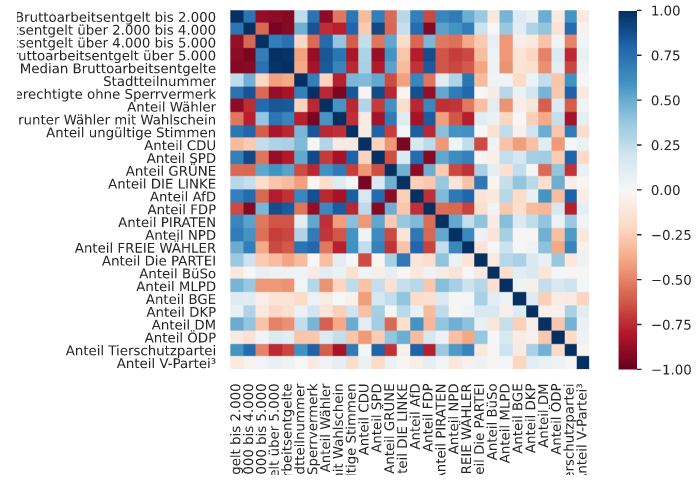
\includegraphics[width=0.8\textwidth]{figure/correlation}
	}
	\caption{Pearson-Korrelation der Daten}
	\label{fig:correlation}
\end{figure}
 stellt die Pearson-Korrelation der Daten da.\\
 Wir wählten anhand der verschiedenen Korrelationstabellen aus den drei unterschiedlichen Reporten verschieden Daten aus, die wir zur Vorhersage verwenden wollten. In die nähere Auswahl fielen schließlich die Daten zum Einkommen und eventuell noch Daten zur Arbeitslosigkeit und Nebenjobdichte. Nach einigen weiteren Untersuchungen dieser Datensätze (zu finden im Ordner "regression", r2 Werte, mögliche lineare Korrelation etc.) auf mögliche Korrelationen dieser Datensätzen zu dem Wahlergebnissen entschieden wir uns für die Einkommensdaten, gegliedert nach Gehaltsgruppen und dem Median (zu finden im "report other").\\     
 
\section{Zielsetzung}
Wir definierten unser Ziel darin, heraus zu finden, ob die beiden unterschiedlichen Algorithmen für eine Prognose des Wahlverhaltens zur Bundestagswahl 2017 in den einzelnen Stadtteilen anhand der Einkommensdaten der Stadtteile in Frankfurt geeignet wären. 

\subsection{Test and verify your data quality}
Im Zusammenhang mit Daten-Qualität existieren unterschiedliche Kriterien. Wichtige sind unter andere Accuracy, Relevancy, Completeness, Timeliness und Consistency (\href{https://towardsdatascience.com/7-steps-to-ensure-and-sustain-data-quality-3c0040591366}{source}). \\
\colorbox{red}{hier könnte man eventuell noch kürzen, wenn nötig}
\begin{description}
\item[Accuracy] Die Daten wurden von der Stadt Frankfurt erhoben und sind damit so akkurat wie möglich. Bei dem mergen der Daten, haben wir sichergestellt, die Bedeutung der Daten nicht zu verändern.
\item[Relevancy] Die von uns verwendeten Daten zu dem Einkommen sind selbstverständlich untereinander korreliert. Nach einigen Untersuchungen mit lediglich dem Median des Einkommens als Datensatz, die zu einer schlechteren Prognose des Wahlverhaltens führten, gehen wir davon aus, dass auch die Einkommensverteilung eine Rolle spielen könnte. Daher erscheinen uns unsere Datenpunkte relevant.
\item[Completeness] Die verwendeten Daten sind nach unserer Bearbeitung bis auf zwei Datensätze in allen Punkten komplett. 
\item[Timeliness] Für eine realistischere Prognose aktueller Wahlen wären sicherlich aktuellere Einkommensdaten sinnvoll. Doch da wir vermuten, dass sich die Einkommensdaten innerhalb weniger Jahre nicht dramatisch ändern und unsere Aufgabe ebenfalls nicht in der Findung eines möglichst guten Vorhersage Modells besteht, sondern wir hier das Vorgehen im Bereich der Data Science darstellen wollen, sind die Daten für unsere Zwecke geeignet.\\
\item[Consitency] Unsere Daten verwenden überall die selben Datentypen und dieselbe Maßeinheiten: Euro für die Angaben des Einkommen und Prozentangaben für das Wahlergebnis. Sie sind in allen Punkten konsistent.
\end{description}


\subsection{Further preprocessing}
Die eben erwähnten Datenpunkte mit fehlenden Werten wurden entfernt. \\ 
\colorbox{red}{unnötig, wir müssen nicht jeden Punkt sklavisch abarbeiten}


\section{Apply two different algorithms of the same kind}
Wir haben zwei ML-Modelle trainiert, Vorhersagen über die Verteilung der Wählerstimmen in Abhängigkeit zu der Einkommensverteilung eines Stadtteils zu treffen.\\
Unsere Target-Values sind der Anteil an den Gesamtstimmen in Prozent (0 - 100\%). Um ein solches Problem zu lösen, bietet sich die  \textit{Multi-Target-Regression} an. scikit-learn stellt solche Funktionalität u.a. mit der Klasse \href{https://scikit-learn.org/stable/modules/generated/sklearn.multioutput.MultiOutputRegressor.html}{MultiOutputRegressor} zur Verfügung. Mit ihr ist es leicht gängige scikit-learn Regressionsmodelle für Multi-Target Probleme zu verwenden. Die zwei von uns getesteten Modelle sind \lstinline|GradientBoostingRegressor| und \lstinline|RandomForestRegressor|.
\begin{description}
	\item[GradientBoosting] baut ein additives Modell schrittweise auf. Es ermöglicht die Optimierung beliebig differenzierbarer Verlustfunktionen. In jeder Stufe wird ein Regressionsbaum an den negativen Gradienten der gegebenen Verlustfunktion angepasst.
	\item[RandomForest] ist ein Meta-Schätzer, der eine Reihe von klassifizierenden Entscheidungsbäumen für verschiedene Teilstichproben des Datensatzes anpasst und mithilfe der Mittelwertbildung die Vorhersagegenauigkeit verbessert und auch Overfitting kontrolliert.	 
\end{description}
 \subsection{Simples Training}
 Für das erste Training wurden die Daten in Training- und Testdaten aufgeteilt. Dafür haben wir die Methode \href{https://scikit-learn.org/stable/modules/generated/sklearn.model_selection.train_test_split.html}{\lstinline|train_test_split|} verwendet. Anschließend wurde über die Methode \lstinline|fit| der Instanzen der Regressorklassen mit den Trainingsdaten die Modelle trainiert. Um die erzeugten Modelle auszuwerten, haben wir uns ihre Vorhersagen für die Testdaten angeschaut. Diese erhält man durch die Methode \lstinline|predict|. Nun können wir auf diese Vorhersage übliche Metriken anwenden. Das Resultat zeigt Tabelle \ref{fig:firstresult}.\\
 \begin{figure}[h]
 	\centering
 	\fbox{	
 		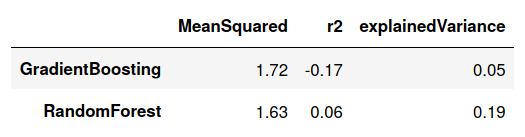
\includegraphics[width=0.6\textwidth]{figure/firstresult}
 	}
 	\caption{Metriken der ersten Modelle}
 	\label{fig:firstresult}
 \end{figure} 
Was bedeuten diese Werte für unsere Modelle?\\
 MeanSquared zeigt den mittleren quadratischen Fehler (MSE) über alle Datenpunkte an. Dieser Wert sag für sich selber nichts über die Güte der Modelle aus, eignet sich aber um verschiedene Modelle miteinander zu vergleichen. Ein niedrigerer Wert ist hier besser. Die Tabelle zeigt, dass RandomForest besser abgeschnitten hat als GradientBoosting.

Die bestmögliche Punktzahl, die bei dem $R^2$ Wert erreicht werden kann, ist 1,0. Ein schlechteres Modell erhält einen kleineren Wert. Dieser Wert kann beliebig negativ werden. Ein konstantes Modell, das unter Berücksichtigung der Eingabemerkmale immer den erwarteten Wert von y vorhersagt, würde einen $R^2$-Wert von 0,0 \textcolor{red}{meinst du hier nicht 1.0?} erhalten. Die Werte beider Modelle sind nahe Null und der von Gradient Boosting sogar negativ. Das Potential beider Modelle, korrekte Vorhersagen zu treffen, scheint also nicht gut zu sein.

Wenn $y$ der Vektor der tatsächlichen Werte ist und $\hat{y}$ die vorhergesagten Werte, dann berechnet $explained\_{}variance(y, \hat{y}) = 1 - \frac{Var\{ y - \hat{y}\}}{Var\{y\}}$. Der beste Wert ist hier wieder 1.0. Üblicherweise sollte ein Modell einen Wert von 0.6 oder höher erreichen, um als valide zu gelten. Davon sind unsere Modelle weit entfernt. Der RandomForest Algorithmus ist minimal besser als der GradientBoosting Algorithmus. 

\subsection{Erneutes Training}
Eine mögliche Ursache für die schlechten Werte könnte sein, dass die Modelle im Training ein niedriges lokales Maxima erreicht haben. Um dies auszuschließen, wiederholen wir das Training auf den selben Daten $n=100$ oft. Abbildung \ref{fig:localminimum}
\begin{figure}[h]
	\centering
	\fbox{	
		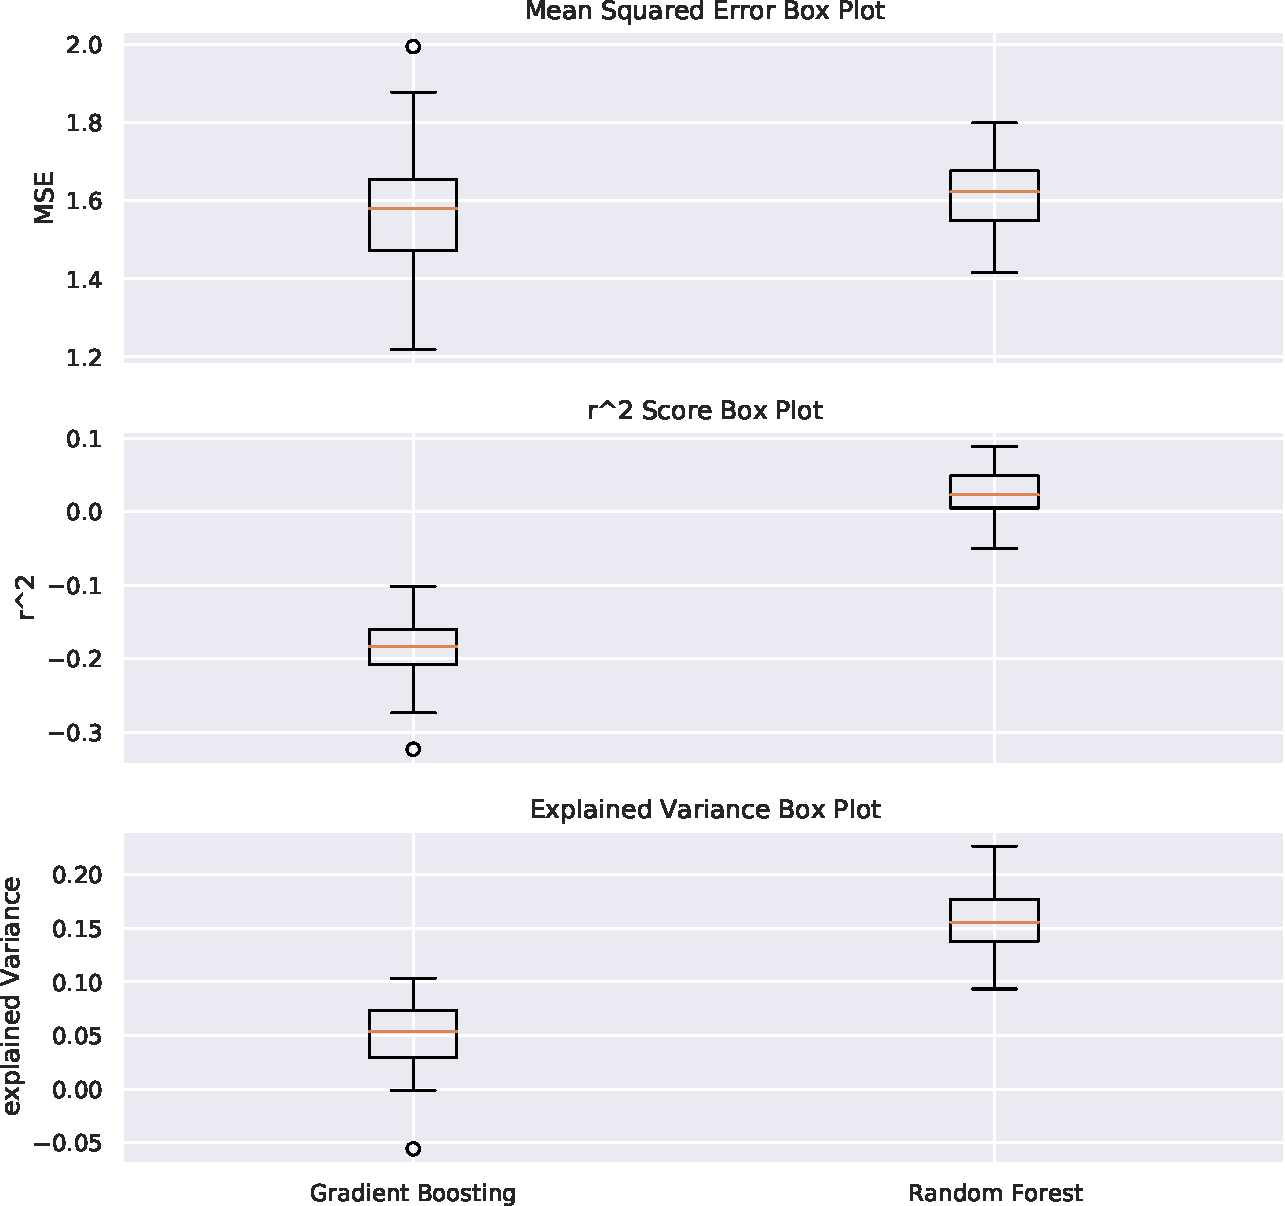
\includegraphics[width=0.6\textwidth]{figure/localminimum}
	}
	\caption{Boxplot der Metriken bei 100 Wiederholungen des Trainings auf denselben Daten}
	\label{fig:localminimum}
\end{figure} 
zeigt das Ergebnis der Auswertung. Auch mit 100 Versuchen erreichten wir keine besseren Werte. Erneut erzielt RandomForest minimal bessere Ergebnisse.
\subsection{Erneutes Training 2.0}
Eine weitere Quelle für ein schlechtes Ergebnis könnte ein schlechte Wahl der Trainingsdaten sein. Ebenfalls relevant könnte unsere eher geringe Menge an Gesamtdaten sein. Daher führten wir das Training mehrfach mit zufälligen Trainingsdaten durch und werteten die Modelle erneut aus. Die dafür verwendete Methode war  \href{https://scikit-learn.org/stable/modules/generated/sklearn.model_selection.cross_validate.html}{\lstinline|cross\_validate|} und das Ergebnis ist in Abbildung \ref{fig:crossval}
\begin{figure}[h]
	\centering
	\fbox{	
		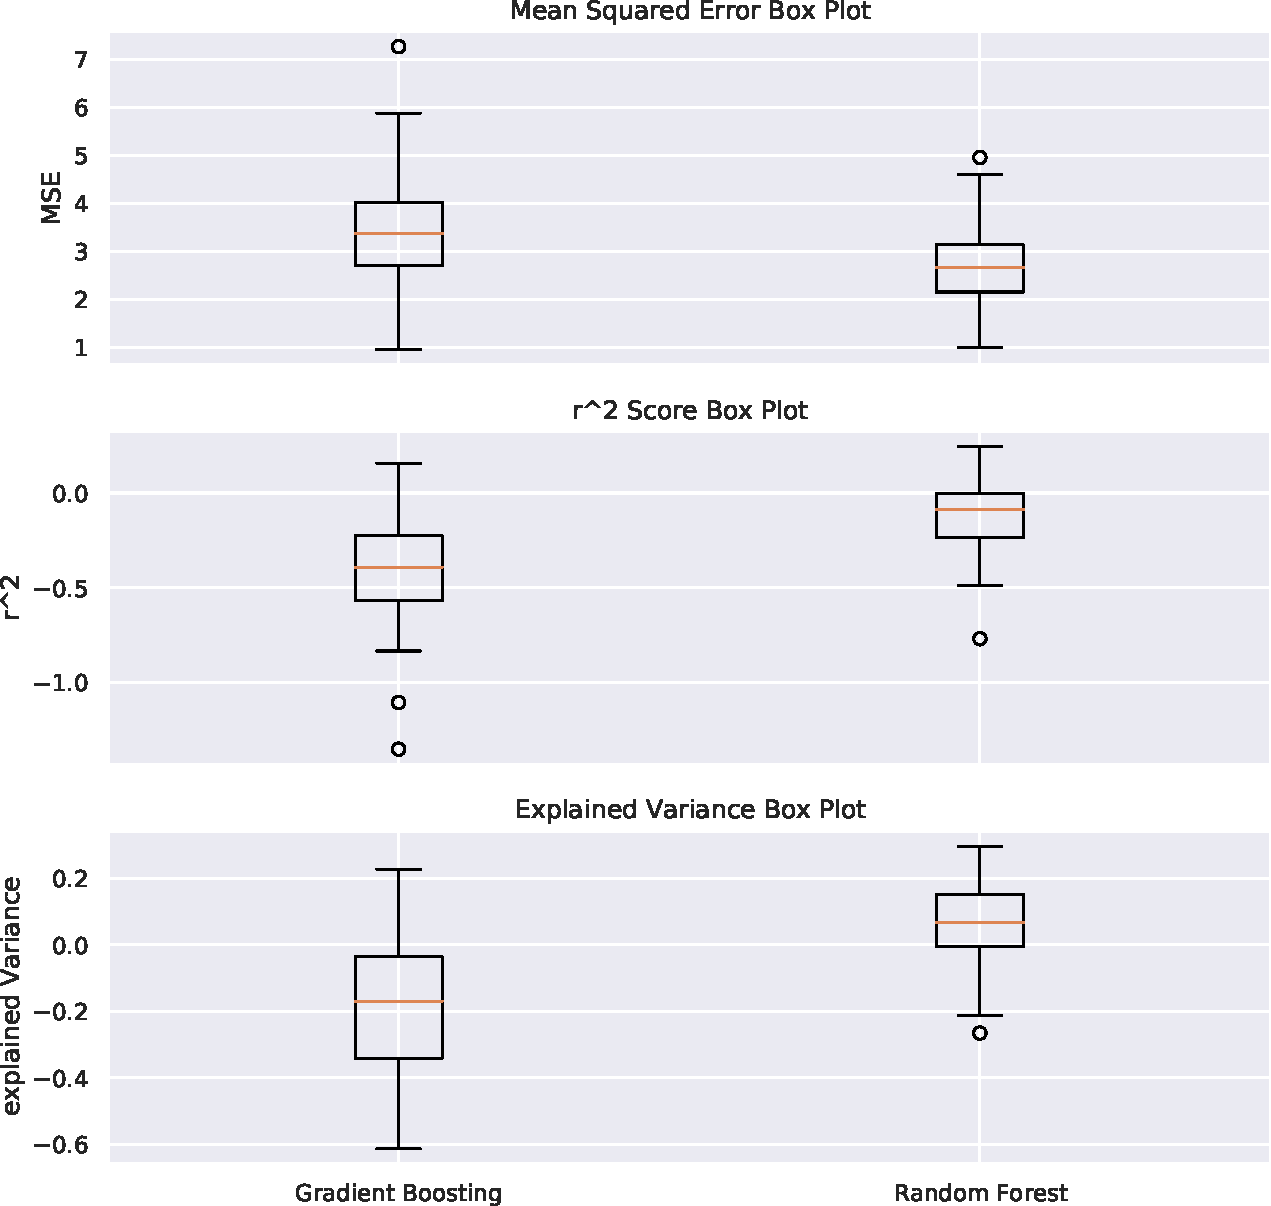
\includegraphics[width=0.6\textwidth]{figure/crossval}
	}
	\caption{Boxplot der Metriken bei 10 Wiederholungen der 5-Fold Cross Validation der Daten}
	\label{fig:crossval}
\end{figure} zu sehen. \\
 Insbesondere an der Verteilung des $R^2$-Scores kann man ablesen, dass beide Modelle in keinem Fall zu wirklich präzisen Ergebnissen führen. 
\subsection{Analyse einzelner Parteien}
Insgesamt machten die Modelle auf uns keinen guten Eindruck. Das schließt aber nicht aus, dass bei bestimmten Parteien nicht Tendenzen erkennen zu sind. Daher unterzogen wir einzelne Parteien einer Analyse. Da uns nicht jede lokale Kleinstpartei interessierte, untersuchten wir nur die wichtigsten Parteien, SPD, CDU, FDP, GRÜNE, DIE LINKE und AFD. Abbildung \ref{fig:simple_parties} \begin{figure}[h]
	\centering
	\fbox{	
		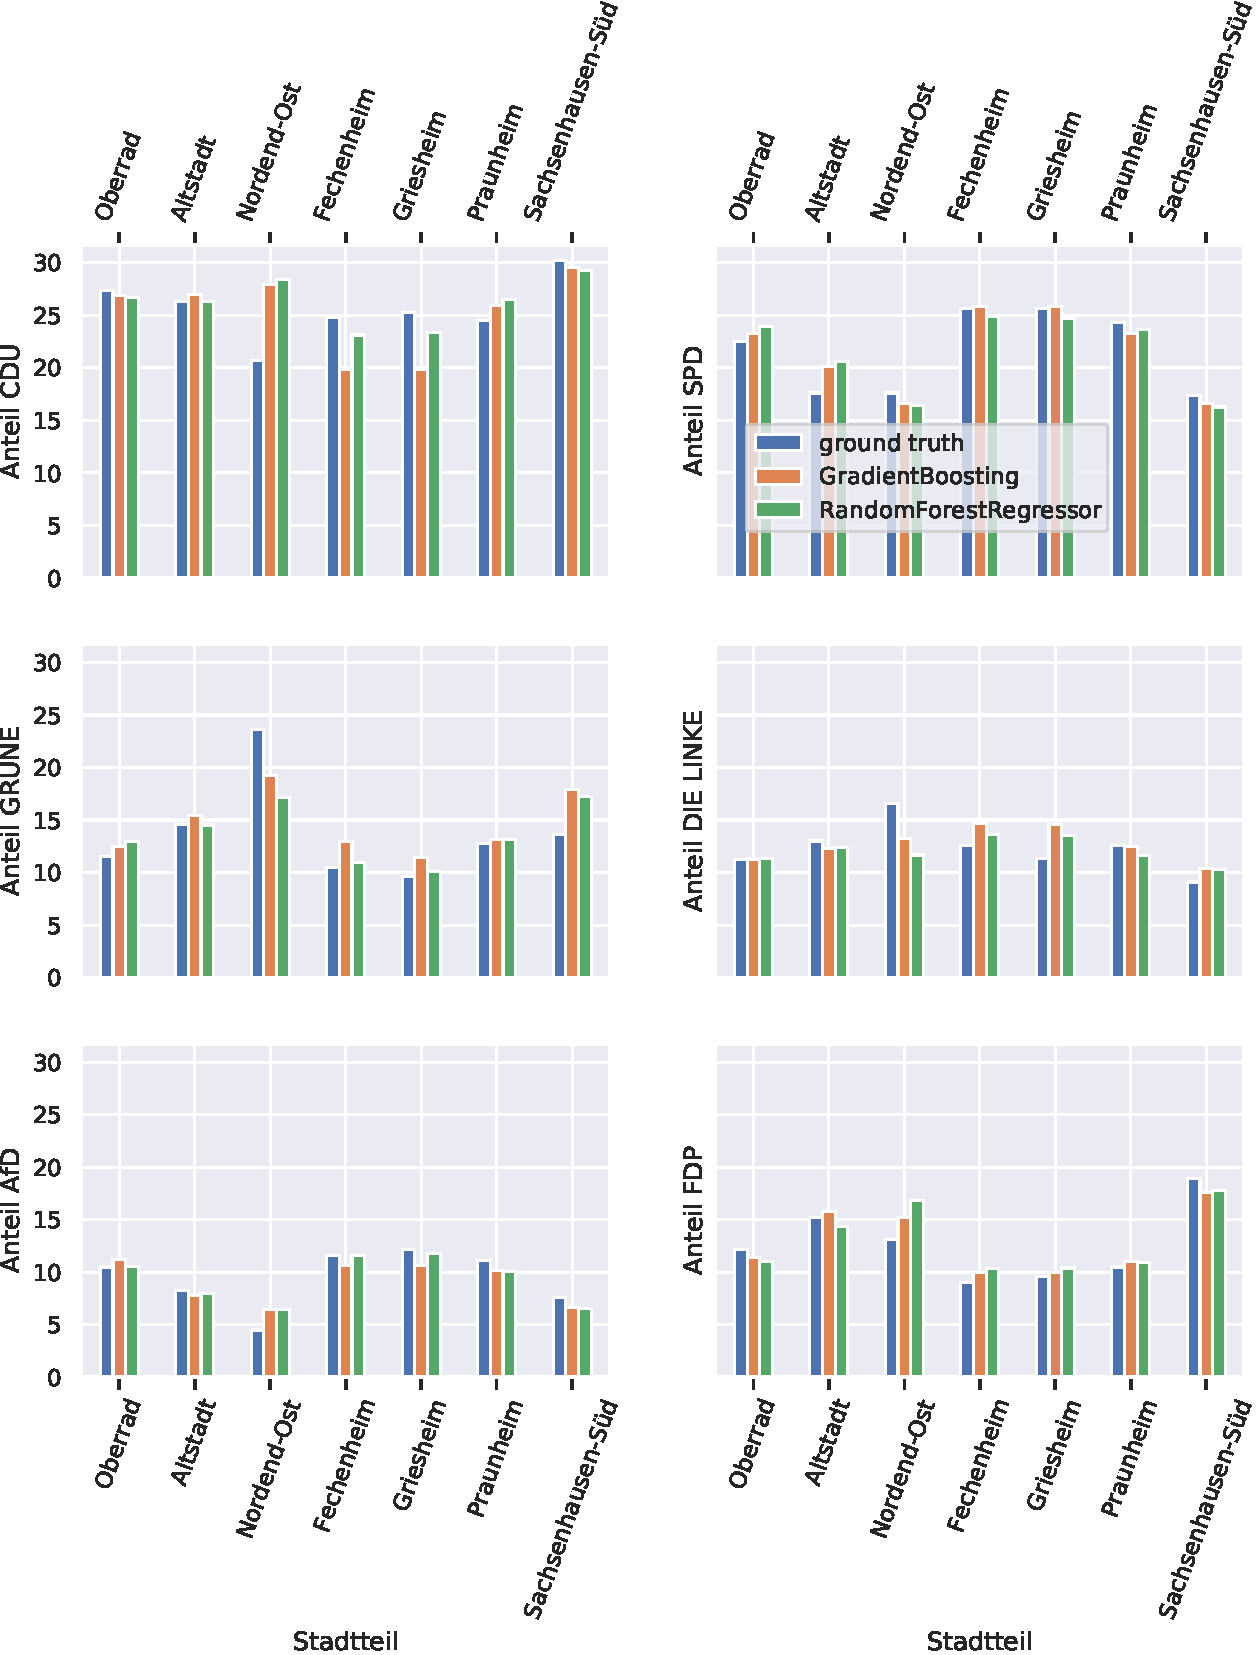
\includegraphics[width=0.9\textwidth]{figure/simple_parties}
	}
	\caption{Vergleich der Vorhersagen zweier Modelle mit der Ground Truth (Auswahl)}
	\label{fig:simple_parties}
	\end{figure}  
	zeigt die Vorhersagen unserer beiden ersten Modelle. Man sieht, die Vorhersagen liegen hier nicht völlig daneben, sie sind nur oft nicht besser als ein konstantes Modell \textcolor{red}{was meinst du mit konstantes Modell?}.

 Nach erneuten Anwendung der Crossvalidation (Abbildung \ref{fig:scores_parties}) \begin{figure}
 	\centering
 	\fbox{	
 		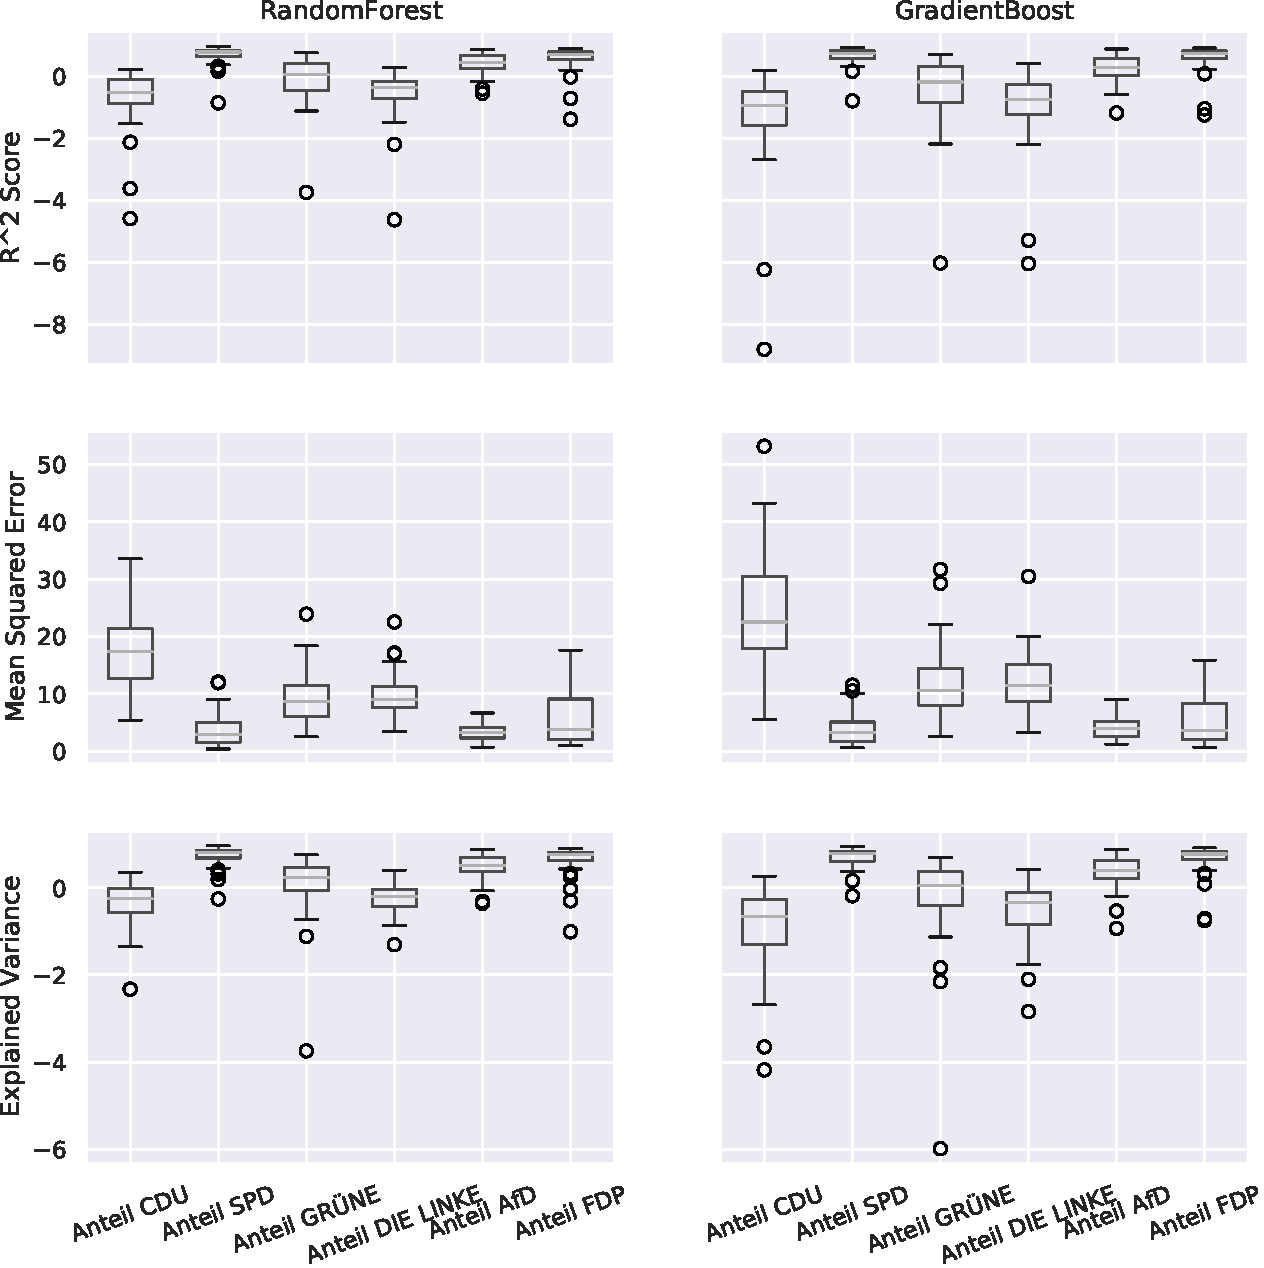
\includegraphics[width=0.9\textwidth]{figure/scores_boxplot_parties}
 	}
 	\caption{Boxplot der Punktzahl verschiedener Metriken der einzelnen Parteien}
 	\label{fig:scores_parties}
 	\end{figure}
 	 fällt ins Auge, dass die Varianz der Werte hoch ist. Die Qualität der Modelle hängt also stark von den zufällig ausgewählten Trainingsdaten ab. Die Menge der Trainingsdaten scheint hier nicht ausreichend zu sein, um ein gutes  Modell zu erstellen. \\
Andererseits sehen wir, dass bei drei Parteien (SPD, DIE LINKE und AFD) im Schnitt die Modelle deutlich besser als ein vergleichbares konstantes Modell sind. Dies können wir daran ablesen, dass dort der $R^2$-Score und die Explained Variance meist höher als 0 sind. Gleichzeitig ist hier der Mean Squared Error deutlich niedriger als für die restlichen Parteien. 
 


\section{Konklusion}
Insagesamt kann man sagen, dass zumindest mit den von uns verwendeten Einkommensdaten und den verwendeten Modellen eine generelle zuverlässige Prognose des Wahlverhaltens eines Stadtteils in Frankfurt nicht möglich ist. Kritisch an den von uns verwendeten Daten könnte sicherlich die zeitliche Differenz der beiden Datensätze und die Korrelation der Eingabe und die Korrelation der Ausgabe Werte untereinander sein, da die von uns verwendeten ML Algorithmen von unabhängigen Parametern ausgehen.\\
 Der Unterschied der Ergebnisse von den beiden Algorithmen ist minimal mit kaum erwähnenswerten Vorteilen für RandomForestRegressor. Vermutlich variieren die von GradientBoostingRegressor gesuchten Maxima zu sehr während RandomForestRegressor etwas davon profitiert, dass er auch Korrelation zwischen Klassen erkennt.  \\
 Für uns überraschend jedoch ist das Ergebnis, dass selbst trotz der eben beschrieben Mängel unser trainiertes Modell für die Parteien DIE LINKE, SPD und AFD bessere Werte liefert als für CDU, FDP und DIE GRÜNEN. Dies legt die Vermutung nahe, dass zumindest für das Ergebnis der ersten drei Parteien die Einkommensverteilung in einem Stadtviertel eine größere Rolle spielt als für letztere.\\
Selbstverständlich war nicht zu erwarten, dass ein so komplexer Prozess wie das Wahlverhalten eines Stadtviertels sich nur anhand der Einkommensverteilung vorhersagen lässt. Es spielen sicherlich aktuelle lokale Geschehnisse, langjährige Parteienbindung und viele andere schwer messbare Faktoren eine entscheidende Rolle. Doch für das Ergebnis einige Parteien hier in Frankfurt scheint die Einkommensverteilung der Wähler eine gewisse Relevanz zu besitzen. 
\end{document}
